\documentclass[11pt]{article}

\usepackage[margin=1.05in]{geometry}
\usepackage{amsmath,amssymb,amsthm,mathtools}
\usepackage{booktabs}
\usepackage{array}
\usepackage{tabularx}
\usepackage{graphicx}
\usepackage{enumitem}
\usepackage{microtype}
\usepackage{xcolor}
\usepackage{tikz}
\usepackage{float}
\usepackage[section]{placeins}
\usetikzlibrary{arrows.meta,calc,fit,positioning,shapes.geometric}
\usepackage[colorlinks=true,linkcolor=blue!55!black,
  citecolor=blue!55!black,urlcolor=blue!55!black]{hyperref}

\newtheorem{theorem}{Theorem}[section]
\newtheorem{definition}[theorem]{Definition}
\newtheorem{lemma}[theorem]{Lemma}
\newtheorem{proposition}[theorem]{Proposition}
\newtheorem{corollary}[theorem]{Corollary}
\newtheorem{remark}[theorem]{Remark}

\newcommand{\lean}[1]{\texttt{#1}}
\newcommand{\code}[1]{\texttt{#1}}
\newcommand{\mergeL}{\mathsf{mergeL}}
\newcommand{\applyop}{\mathsf{apply}}
\newcommand{\init}{\sigma_0}
\newcommand{\events}{\mathcal E}
\newcommand{\state}{\Sigma}
\newcommand{\vis}{\mathrel{\mathsf{vis}}}
\newcommand{\lo}{\mathsf{lo}}
\newcommand{\erase}{\mathsf{erase}}
\newcommand{\cfg}{\mathcal C}
\newcommand{\versions}{\mathcal V}
\newcommand{\heads}{\mathcal H}
\newcommand{\parents}{\mathcal P}
\newcommand{\Rule}[3]{%
  \frac{\begin{array}{c}#2\end{array}}{#3}\;\textsc{#1}}
\newcommand{\smallcode}[1]{\texttt{\small #1}}

\tikzset{
  version/.style={circle,draw,minimum size=5.5mm,inner sep=0pt,font=\small},
  ghost/.style={version,dashed},
  replica/.style={rectangle,rounded corners,draw,inner sep=3pt,font=\small},
  flow/.style={-{Latex[length=2mm]},semithick},
  data/.style={rectangle,rounded corners,draw,align=center,inner sep=5pt},
  theoremnode/.style={rectangle,rounded corners,draw=blue!55!black,
    fill=blue!4,align=center,inner sep=5pt},
  certnode/.style={rectangle,rounded corners,draw=orange!70!black,
    fill=orange!5,align=center,inner sep=5pt}
}

\setlist{nosep}
\sloppy


\title{A Corrected Metatheory for Mergeable Replicated Data Types}
\author{Anonymous Authors}
\date{}
\hypersetup{pdftitle={A Corrected Metatheory for Mergeable Replicated Data Types},
  pdfauthor={Anonymous Authors},bookmarksopen=true,bookmarksnumbered=true}

\begin{document}
\maketitle

\begin{abstract}
Mergeable replicated data types reconcile two branch states relative to a
common ancestor. The original bottom-up linearization argument for this model
does not hold: a global arbitration relation can change when an event outside
the version being linearized absorbs an edge. We give a corrected Lean~4
metatheory based on set-relative arbitration, a reachable store invariant, and
a contextual ternary Join lemma. We keep the operational MRDT signature free
of client invariants and applicability fields. Datatype implementers instead
supply generation, convergence, sequential-refinement, and safety
certificates. The framework also supplies canonical virtual LCAs and an
asynchronous distributed collector for commit history. Datatype-state garbage
collection is optional and composes with the history collector by trace
erasure. All theorem names in this paper are checked by the repository's
\lean{RefactorLedger.lean} build target.
\end{abstract}

\tableofcontents

\section{Result and evidence boundary}

An MRDT stores immutable versions in a Git-like directed acyclic graph. An
update extends one replica head. A merge of branch states $a$ and $b$ reads the
state $l$ at their common ancestor and computes $\mergeL(l,a,b)$. The client
expects the state at every registered version to equal a legal sequential fold
of exactly that version's events.

Figure~\ref{fig:execution-shape} is the running execution shape. The graph is
not decoration: apply creates a one-parent version, merge creates a two-parent
version, and a later merge may use an old version as its base. This is why the
correctness invariant ranges over the store rather than only the current
heads.

\begin{figure}[t]
\centering
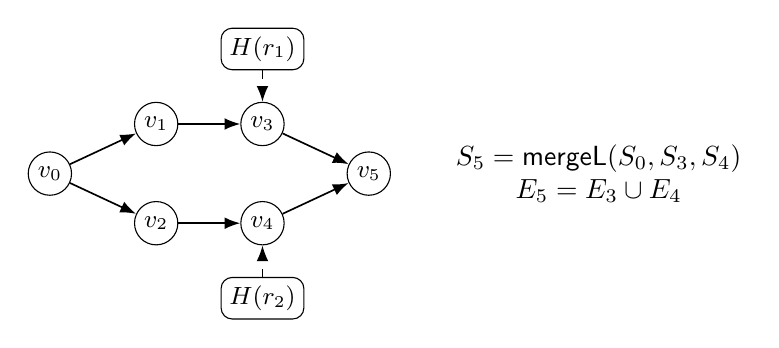
\begin{tikzpicture}[x=1.35cm,y=0.9cm]
  \node[version] (v0) at (0,0) {$v_0$};
  \node[version] (v1) at (1,0.7) {$v_1$};
  \node[version] (v2) at (1,-0.7) {$v_2$};
  \node[version] (v3) at (2,0.7) {$v_3$};
  \node[version] (v4) at (2,-0.7) {$v_4$};
  \node[version] (v5) at (3,0) {$v_5$};
  \draw[flow] (v0)--(v1); \draw[flow] (v0)--(v2);
  \draw[flow] (v1)--(v3); \draw[flow] (v2)--(v4);
  \draw[flow] (v3)--(v5); \draw[flow] (v4)--(v5);
  \node[replica,above=4mm of v3] (r1) {$H(r_1)$};
  \node[replica,below=4mm of v4] (r2) {$H(r_2)$};
  \draw[flow,dashed] (r1)--(v3); \draw[flow,dashed] (r2)--(v4);
  \node[align=center,right=7mm of v5] {$S_5=\mergeL(S_0,S_3,S_4)$\\
    $E_5=E_3\cup E_4$};
\end{tikzpicture}
\caption{A version-DAG execution. Solid arrows point from parents to
children. The merge at $v_5$ reads the registered LCA $v_0$ and both branch
heads.}
\label{fig:execution-shape}
\end{figure}

The current artifact separates four kinds of evidence.

\begin{center}
\begin{tabular}{@{}lll@{}}
\toprule
Layer & Framework supplies & Datatype supplies \\
\midrule
Raw execution & version DAG, apply, merge, query & state and operations \\
Convergence & canonical adequacy, virtual LCA & contextual Join proof \\
Client protocol & guarded execution & generation guard and history bridge \\
Client meaning & certificate interfaces & sequential and safety proofs \\
Commit GC & distributed protocol and refinement & none \\
State GC & generic trace-erasure theorem & optional physical protocol \\
\bottomrule
\end{tabular}
\end{center}

This boundary matters. A theorem about a semantic MRDT does not by itself
verify an editor widget, a wire decoder, or crash recovery. The JavaScript
runtime is tested against the model-facing fixtures, but it is not extracted
from Lean. We call Lean declarations \emph{machine-checked}, runtime test
results \emph{validated}, and benchmark observations \emph{measured}.

\section{Raw MRDT semantics}

\subsection{The signature stays plain}

\begin{definition}[MRDT signature]
An MRDT signature contains a state type $\state$, initial state $\init$,
application operation, query interface, conflict-resolution relation, binary
merge inherited from the CRDT core, and ternary merge
\[
  \mergeL : \state \to \state \to \state \to \state.
\]
The compatibility law $\mergeL(\init,a,b)=\mathsf{merge}(a,b)$ relates the
ternary and initial-slice binary operations.
\hfill\lean{MRDTSig}
\end{definition}

The signature has no fields named invariant or applicable. A client can invoke
the raw update on every state. Generation restrictions enter only in the
certified execution of Section~\ref{sec:generation}. This choice prevents the
datatype carrier, client protocol, and safety theorem from becoming one
circular definition.

The optional \lean{LocalCommutationDomain} is a proof aid for algorithms whose
updates commute only under local hypotheses. It does not restrict raw
execution and is not required by \lean{VerifiedMRDT}.

\subsection{Configurations and transitions}

A paper-level configuration is
\[
  C=\langle V,H,P,\vis\rangle,
  \qquad V(v)=(S_v,E_v),
\]
where $V$ is the finite version store, $H$ maps replicas to heads, $P$ maps a
version to its parents, and $\vis$ is event visibility. Replica state and
replica events are derived as $S_{H(r)}$ and $E_{H(r)}$. The Lean
\lean{Configuration} also caches these two projections as \lean{N} and
\lean{L}; \lean{head\_coherent} requires the caches to equal the derivation
above. We omit the caches from the rules because they contain no independent
semantic information.

Version numbers increase along parent edges. The configuration requires
immutable event timestamps, per-replica causal order, coherent heads, and the
key LCA equation:
if $v_T$ is an LCA of $v_1$ and $v_2$, then
\[
  \events(v_T)=\events(v_1)\cap\events(v_2).
\]

Figure~\ref{fig:raw-semantics} gives the state-changing core of \lean{Step}.
The notation $C[v\mapsto(S,E);r\mapsto v;P(v)\mapsto\pi]$ updates the version
store, replica head, and parent list while preserving all other entries.
\textsc{Query} returns $\mathsf{query}(S_{H(r)},q)$ without changing $C$;
\textsc{Create} installs the initial version at a fresh replica. The raw
\textsc{Apply} rule deliberately does not check a datatype-specific client
guard.

\begin{figure}[t]
\small
\[
\Rule{Apply}{
  H(r)=v \quad V(v)=(S,E) \quad t\notin\mathsf{times}(C)
  \\
  v'\notin\mathsf{dom}(V) \quad v<v' \quad e=(t,r,o)
}{
  C\xrightarrow{\mathsf{apply}(t,r,o)}
  C[v'\mapsto(\mathsf{do}(S,e),E\cup\{e\});
    r\mapsto v';P(v')\mapsto[v]]
}
\]
\[
\Rule{Merge}{
  H(r_1)=v_1 \quad H(r_2)=v_2 \quad
  \mathsf{LCA}_P(v_1,v_2)=v_T
  \\
  V(v_i)=(S_i,E_i)\ (i\in\{1,2,T\}) \quad
  v_m\notin\mathsf{dom}(V) \quad v_1,v_2<v_m
}{
  C\xrightarrow{\mathsf{merge}(r_1,r_2)}
  C[v_m\mapsto(\mergeL(S_T,S_1,S_2),E_1\cup E_2);
    r_1\mapsto v_m;P(v_m)\mapsto[v_1,v_2]]
}
\]
\caption{Paper-level raw operational semantics. The Lean rules also update
the coherent replica caches and extend visibility on apply.}
\label{fig:raw-semantics}
\end{figure}

\section{Why the earlier induction fails}

The conflict relation induces an arbitration order $\lo$. The first proof
attempt used a relation computed from the entire configuration while
linearizing a smaller version event set. That is unsound when a third event,
outside the smaller set, absorbs an arbitration edge.

\begin{proposition}[global-order convergence is false]
There is a two-operation add-wins signature and a legal configuration with a
backward-closed event set $E$ such that two enumerations of $E$ both respect
the configuration-global arbitration relation but fold to different states.
\hfill\lean{convergence\_over\_backward\_closed\_subsets\_false}
\end{proposition}

The checked countermodel is in
\code{Metatheory/Join/Convergence\_CounterModel.lean}. The repaired relation
\lean{loOn C E} computes arbitration relative to $E$. In the countermodel it
retains the edge that the outside absorber erased globally.

Associativity, commutativity, and idempotence of merge do not repair the proof.
The second checked countermodel satisfies the core update laws and a bounded
join-semilattice merge but violates both the peel laws and the Join lemma.
\hfill\lean{coreVCs\_lattice\_insufficient}

These countermodels establish two boundaries: arbitration must be local to the
set being linearized, and convergence needs a contextual bridge between merge
and update history.

Figure~\ref{fig:proof-repair} summarizes the repair. The failed path tried to
peel operations from a merge using a global order. The checked path instead
proves canonicality for each stored event set and uses one contextual Join
obligation at every merge.

\begin{figure}[t]
\centering
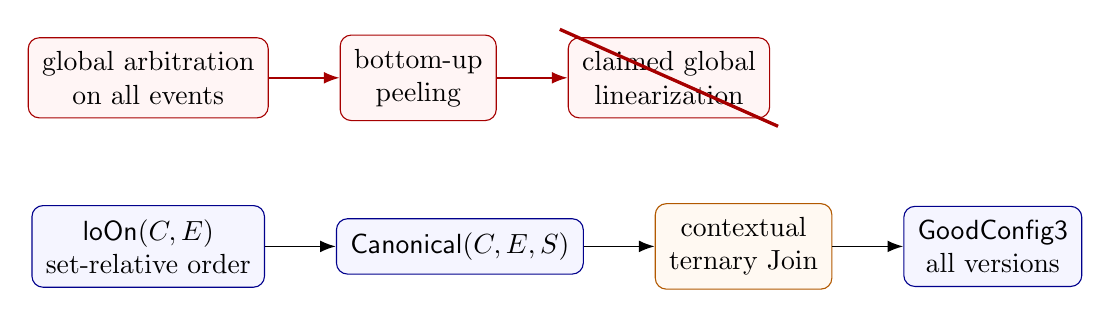
\begin{tikzpicture}[node distance=7mm and 9mm]
  \node[data,draw=red!65!black,fill=red!4] (global) {global arbitration\\on all events};
  \node[data,draw=red!65!black,fill=red!4,right=of global] (peel) {bottom-up\\peeling};
  \node[data,draw=red!65!black,fill=red!4,right=of peel] (bad) {claimed global\\linearization};
  \draw[flow,red!65!black] (global)--(peel);
  \draw[flow,red!65!black] (peel)--(bad);
  \draw[red!65!black,very thick] ($(bad.north west)+(-1mm,1mm)$)--($(bad.south east)+(1mm,-1mm)$);

  \node[theoremnode,below=11mm of global] (local) {$\mathsf{loOn}(C,E)$\\set-relative order};
  \node[theoremnode,right=of local] (canon) {$\mathsf{Canonical}(C,E,S)$};
  \node[certnode,right=of canon] (join) {contextual\\ternary Join};
  \node[theoremnode,right=of join] (good) {$\mathsf{GoodConfig3}$\\all versions};
  \draw[flow] (local)--(canon); \draw[flow] (canon)--(join); \draw[flow] (join)--(good);
\end{tikzpicture}
\caption{The failed bottom-up argument and the checked canonical-adequacy
argument. Red nodes describe the refuted route; blue/orange nodes are current
Lean interfaces and invariants.}
\label{fig:proof-repair}
\end{figure}

\section{Canonical adequacy}

\subsection{Canonical states}

For configuration $C$ and event set $E$, a state is canonical when some
duplicate-free enumeration of exactly $E$ respects \lean{loOn C E} and folds
from $\init$ to that state. The update-layer lemmas prove that any two such
enumerations have the same fold under the supplied update conditions.

The reachable invariant \lean{GoodConfig3} states that every registered
version contains a canonical state of its event set. It also retains
visibility transitivity and irreflexivity, event support, and causal closure.
The invariant ranges over all versions, not only replica heads, because later
merges may read an older version as their LCA.

\subsection{The ternary Join obligation}

\begin{definition}[contextual ternary Join]
For a configuration $C$, suppose $E_1$ and $E_2$ satisfy the required closure
conditions. If $s_0$, $s_1$, and $s_2$ are canonical for
$E_1\cap E_2$, $E_1$, and $E_2$, respectively, then
\[
  \mergeL(s_0,s_1,s_2)
\]
must be canonical for $E_1\cup E_2$.
\hfill\lean{JoinLemma3At}
\end{definition}

\lean{JoinLemma3} quantifies this obligation over all configurations. Some
datatypes prove the weaker per-configuration form from a history fact. The
full-closure sibling \lean{JoinLemma3F} supports algorithms whose merge proof
needs complete causal closure rather than only non-commuting predecessors.

\begin{theorem}[ordinary adequacy]
If a datatype satisfies \lean{JoinLemma3}, every configuration reachable from
\lean{initConfig} by \lean{Step} is RA-linearizable at every registered
version.
\hfill\lean{ra\_linearizable3\_of\_join}
\end{theorem}

The proof carries \lean{StoreInv} with \lean{GoodConfig3}. The store invariant
proves that parent reachability remains well founded and that the selected LCA
contains exactly the event-set intersection
(\lean{lca\_events\_of\_storeInv}). Apply extends a canonical fold by a fresh
event. Merge invokes the Join obligation. Query and replica creation preserve
the invariant directly.

The framework retains the eight-condition route as one constructor for Join:
\lean{CoreVCs3CD}, \lean{FeasibleDeltaVCs3}, and \lean{CDVC3} imply
\lean{JoinLemma3}. Datatypes may instead prove Join directly; the public
\lean{VerifiedMRDT} package depends on the convergence result, not on one
particular VC decomposition.

\section{Generation, sequential meaning, and safety}
\label{sec:generation}

RGA insertion illustrates why a plain signature still needs a client
protocol. An insertion carries an anchor and a fresh identifier. Raw delivery
can apply that record anywhere, but honest minting requires the issuer to have
seen the anchor and to choose an identifier above its causal past. This is a
historical fact about the minting state, not a shape predicate on an arbitrary
later delivery state.

\begin{definition}[generation contract]
A \lean{GenerationContract D} contains
\[
\begin{array}{ll}
\mathsf{Guard} &: \mathsf{Op}\to\state\to\mathsf{Prop},\\
\mathsf{History} &: \mathsf{Configuration}\to\mathsf{Prop},\\
\mathsf{history\_of\_mint} &: \mathsf{MintHonest}(\mathsf{Guard},C)
  \to \mathsf{History}(C).
\end{array}
\]
\end{definition}

\lean{GuardedStep} checks the guard only for an apply transition and checks it
at the issuer's current materialized head. Non-apply transitions retain their
raw semantics. A final configuration does not store all former issuer heads,
so \lean{MintCertifiedReach} explicitly carries a causal-fold mint witness at
each step. \lean{MintCertifiedReachV} is the virtual-LCA counterpart.

\begin{figure}[t]
\small
\[
\Rule{Certified-Apply}{
  C\xrightarrow{\mathsf{apply}(t,r,o)}C' \quad H(r)=v
  \quad V(v)=(S,E) \quad G.\mathsf{Guard}((t,r,o),S)
}{
  C\xRightarrow[G]{\mathsf{apply}(t,r,o)}C'
}
\]
\[
\Rule{Certified-Other}{
  C\xrightarrow{\ell}C' \quad \ell\ne\mathsf{apply}(-,-,-)
}{
  C\xRightarrow[G]{\ell}C'
}
\]
\caption{Generation-certified execution. Certification restricts minting at
the issuer head; it does not alter raw delivery or merge semantics. A
\lean{MintCertifiedReach} trace additionally retains the historical mint
witness needed after the issuer moves to a later head.}
\label{fig:certified-semantics}
\end{figure}

\begin{definition}[verified MRDT]
An implementer supplies:
\begin{itemize}
\item a \lean{GenerationContract};
\item a \lean{ConvergenceCertificate} for ordinary and virtual-LCA certified
  executions;
\item an independent \lean{SequentialSpec} and \lean{SequentialRefinement};
\item a bridge from \lean{LinearMintHistory} to the sequential honesty
  predicate; and
\item a \lean{SafetyCertificate} with a state invariant, its preservation on
  ordinary and virtual certified executions, and an observable consequence.
\end{itemize}
\hfill\lean{VerifiedMRDT}
\end{definition}

The package exposes three capstones:
\lean{VerifiedMRDT.converges}, \lean{VerifiedMRDT.convergesV}, and
\lean{VerifiedMRDT.sequentially\_correct}. The safety certificate remains
separate because convergence does not imply a client invariant. For example,
the bounded counter proves non-negative observable values through a global
history invariant; arbitrary ternary tuples do not preserve that invariant.

\section{Canonical virtual LCAs}

Criss-cross histories can have several maximal common ancestors and no unique
registered LCA. Choosing one maximal ancestor can lose events represented by
another. The framework instead constructs a synthetic state by recursively
folding the maximal-common-ancestor frontier.

\lean{canonicalVirtualLCA} implements this resolver. The support decreases
under the version order, which justifies the recursion. The key theorem
\lean{virtualLCAState\_canonical} proves that the synthetic state is canonical
for the union of the maximal ancestors' event sets. The store theorem
\lean{mca\_events\_cover} shows that this union covers every common ancestor.

\lean{StepV} conservatively embeds every ordinary \lean{Step} and adds one
virtual merge constructor. It allocates only the resulting version; the
synthetic base is ghost semantic state.

\begin{theorem}[virtual-LCA adequacy]
The same \lean{JoinLemma3} that proves ordinary adequacy proves
RA-linearizability for configurations reachable under \lean{StepV} with the
canonical resolver.
\hfill\lean{ra\_linearizable3V\_of\_join}
\end{theorem}

No new datatype merge law is introduced by virtual LCAs.

\begin{figure}[t]
\centering
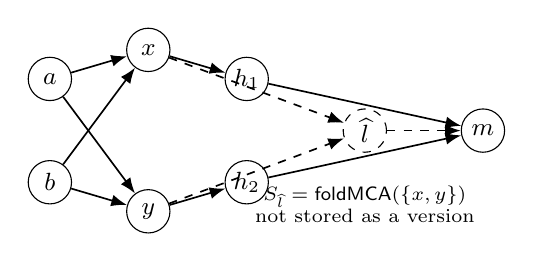
\begin{tikzpicture}[x=1.25cm,y=0.82cm]
  \node[version] (a) at (0,0.8) {$a$};
  \node[version] (b) at (0,-0.8) {$b$};
  \node[version] (x) at (1,1.25) {$x$};
  \node[version] (y) at (1,-1.25) {$y$};
  \node[version] (h1) at (2,0.8) {$h_1$};
  \node[version] (h2) at (2,-0.8) {$h_2$};
  \node[ghost] (vlca) at (3.2,0) {$\widehat l$};
  \node[version] (m) at (4.4,0) {$m$};
  \draw[flow] (a)--(x); \draw[flow] (a)--(y);
  \draw[flow] (b)--(x); \draw[flow] (b)--(y);
  \draw[flow] (x)--(h1); \draw[flow] (y)--(h2);
  \draw[flow,dashed] (x)--(vlca); \draw[flow,dashed] (y)--(vlca);
  \draw[flow,dashed] (vlca)--(m); \draw[flow] (h1)--(m); \draw[flow] (h2)--(m);
  \node[align=center,below=3mm of vlca,font=\scriptsize]
    {$S_{\widehat l}=\mathsf{foldMCA}(\{x,y\})$\\not stored as a version};
\end{tikzpicture}
\caption{A criss-cross history has two maximal common ancestors, $x$ and
$y$. The canonical virtual LCA is ghost state. Only the merge result $m$ is
allocated.}
\label{fig:virtual-lca}
\end{figure}

\section{Distributed commit-history garbage collection}

Commit-history GC belongs to the runtime framework. It is not supplied once
per datatype, and the public framework has no global stop-the-world collector.

\subsection{Minimal local state}

For each replica, the logical collector stores only
\[
  L=\{\mathsf{head}:\mathit{Version},\quad
      \mathsf{commits}:\mathcal P(\mathit{Version})\},
  \qquad \mathsf{head}\in\mathsf{commits}.
\]
The parent relation, fixed roster, and immutable optional author of each
operation commit are protocol parameters. Roots and merge commits are
unauthored. An envelope contains only a commit set. Fetch is set union and does
not change the receiving head; head synchronization is a separate transition.
\hfill\lean{GC.Local}, \lean{GC.Envelope}

Evidence is derived rather than stored. Replica $r$ has frontier evidence at
$L$ when $L$ retains a commit authored by $r$ that reaches $L.\mathsf{head}$.
\lean{GC.EvidenceComplete} requires such evidence for every other roster
member. The negative control \lean{GC.EvidenceSPOT.missing\_author} confirms
that an unauthored merge head cannot stand in for a missing author's evidence.

\subsection{Collection certificate}

A \lean{GC.Certificate} supplies a keep set containing the local head and the
evidence witnesses. It proves support in the local holding and exact
reachability and LCA answers between retained versions. The canonical
constructor \lean{GC.Certificate.ofMCAClosed} uses a keep set closed under
maximal common ancestors.

The compressed graph connects two retained versions when the original graph
reached between them. It need not retain intermediate paths or the old root.
\lean{GC.compressedReaches\_iff} proves reachability equivalence, and
\lean{GC.root\_absent\_when\_dropped} proves that a root outside the keep set
is absent from the retained carrier.

\subsection{Direct asynchronous refinement}

The collecting protocol has fetch, head synchronization, and local GC. Its
no-GC counterpart has the same network steps and no collection transition.
The simulation relates one full and one compact local store by equal heads and
commit-set inclusion.

\begin{figure}[t]
\small
\[
\Rule{Fetch}{
  M=\mathsf{commits}(W(s))
}{
  W\longrightarrow W[d\mapsto
    \langle\mathsf{head}(W(d)),\mathsf{commits}(W(d))\cup M\rangle]
}
\]
\[
\Rule{Head-Sync}{v\in\mathsf{commits}(W(r))}{
  W\longrightarrow W[r\mapsto
    \langle v,\mathsf{commits}(W(r))\rangle]}
\qquad
\Rule{Collect}{\mathsf{Certificate}(W(r),K)}{
  W\longrightarrow W[r\mapsto\langle\mathsf{head}(W(r)),K\rangle]}
\]
\caption{Asynchronous commit-history GC. Fetch is the ordinary remote-fetch
path and unions immutable commits. Head synchronization is explicit. Collect
is local and requires complete frontier evidence plus reachability/LCA
preservation for the keep set.}
\label{fig:distributed-gc-rules}
\end{figure}

\begin{theorem}[distributed collection refines no-GC]
Every finite collecting execution is matched by a finite no-GC execution.
Fetch and head synchronization match their counterparts; collection
stutters. The final worlds have equal replica heads, so head-state reads are
unchanged.
\hfill\lean{GC.execution\_refines\_noGC}, \lean{GC.read\_preserved}
\end{theorem}

The runtime lifting adds a ghost MRDT configuration to state the semantic
simulation. Visible apply and merge labels evolve that configuration. Fetch
and GC remain silent. Erasing silent labels yields an ordinary or virtual-LCA
core execution
(\lean{GC.runtime\_refines\_core}, \lean{GC.runtime\_refines\_coreV}). The
ghost configuration is not a second physical copy required of an
implementation.

\section{Optional datatype-state garbage collection}

Commit GC removes versions from a replica's history. It cannot decide whether
an RGA tombstone, a Peritext mark boundary, or a TreeMove event can be removed
from the state stored at a retained version. That decision is datatype
specific.

\begin{definition}[state-GC protocol]
A \lean{StateGCProtocol} supplies a physical state, a projection to a semantic
configuration, a validity predicate, and physical transitions labelled by an
optional semantic label. It proves:
\begin{enumerate}
\item validity is invariant;
\item a silent physical transition leaves the semantic projection unchanged;
\item a visible transition refines a \lean{StepV} transition.
\end{enumerate}
\end{definition}

\begin{theorem}[state collection refines semantic execution]
Erasing silent labels from any valid finite physical trace yields a finite
\lean{StepV} trace between the projected configurations.
\hfill\lean{StateGCProtocol.refines}
\end{theorem}

The combined physical state contains the datatype protocol state and the
generic distributed commit stores. A combined transition is either a datatype
physical step or a silent fetch/commit-GC step.

\begin{theorem}[the two collectors compose]
For every valid finite combined trace, erasing state-GC, fetch, and commit-GC
labels yields an execution of the uncollected virtual-LCA semantics.
\hfill\lean{GC.CombinedSteps.refinesV}
\end{theorem}

The ordinary corollary \lean{GC.CombinedSteps.refinesRaw} applies when every
visible datatype transition proves a raw \lean{Step}. Sided Peritext and
TreeMove provide concrete state-GC protocols. Other datatypes may omit the
interface entirely.

\begin{figure}[t]
\centering
\resizebox{\textwidth}{!}{%
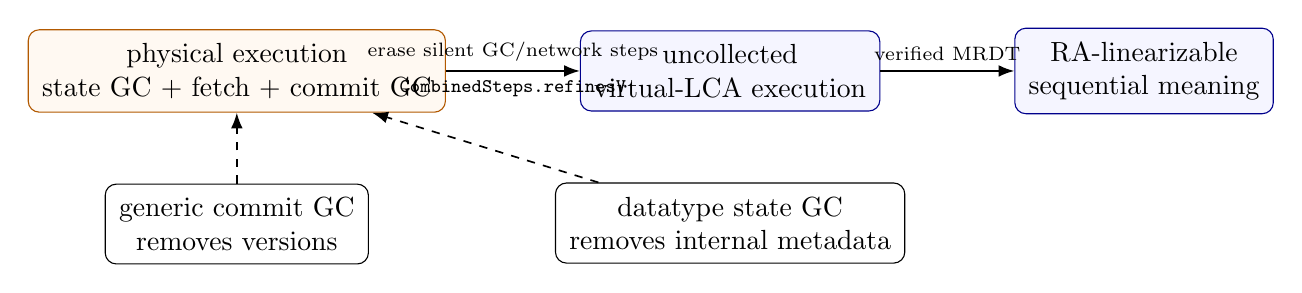
\begin{tikzpicture}[node distance=9mm and 17mm]
  \node[certnode] (physical) {physical execution\\state GC + fetch + commit GC};
  \node[theoremnode,right=of physical] (virtual) {uncollected\\virtual-LCA execution};
  \node[theoremnode,right=of virtual] (raw) {RA-linearizable\\sequential meaning};
  \draw[flow] (physical)--node[above,font=\scriptsize]{erase silent GC/network steps}
    node[below,font=\scriptsize]{\lean{CombinedSteps.refinesV}}(virtual);
  \draw[flow] (virtual)--node[above,font=\scriptsize]{verified MRDT}(raw);
  \node[data,below=9mm of physical] (history) {generic commit GC\\removes versions};
  \node[data,below=9mm of virtual] (state) {datatype state GC\\removes internal metadata};
  \draw[flow,dashed] (history)--(physical);
  \draw[flow,dashed] (state)--(physical);
\end{tikzpicture}
}
\caption{The two collectors remove different objects and compose by trace
erasure. Neither collector changes the visible MRDT semantics.}
\label{fig:two-gc-composition}
\end{figure}

\section{Machine-checked instances}

Table~\ref{tab:instances} lists the packages imported by
\lean{Metatheory/RefactorLedger.lean}. A checkmark means that the current Lean
tree contains the named public package; it does not claim that the JavaScript
runtime is extracted from that package.

\begin{table}[h]
\centering
\small
\begin{tabular}{@{}lcccc@{}}
\toprule
Datatype & Generation & Convergence & Sequential & State GC \\
\midrule
Bounded counter & \checkmark & \checkmark & \checkmark & -- \\
RGA with tombstones & \checkmark & \checkmark & \checkmark & -- \\
EmbedRGA & \checkmark & \checkmark & \checkmark & policy lemmas \\
SidedEmbedRGA/FugueMax & \checkmark & \checkmark & \checkmark & policy lemmas \\
MVR & \checkmark & \checkmark & \checkmark & -- \\
Mergeable queue & \checkmark & \checkmark & \checkmark & -- \\
Peritext & \checkmark & \checkmark & \checkmark & concrete protocol \\
TreeMove & \checkmark & \checkmark & \checkmark & concrete protocol \\
\bottomrule
\end{tabular}
\caption{Current nontrivial certificate packages. Trivial-generation
grow-only and counter products are also in the ledger.}
\label{tab:instances}
\end{table}

The production ledger also checks product construction, Fugue and FugueMax
non-interleaving results, Peritext rendering, the distributed collector, and
the combined GC theorem. It is an import-and-name gate rather than an axiom
eliminator. The cited instance files print standard Lean axioms only; the
repository release script separately rejects \lean{sorry} and
\lean{sorryAx} in the production tree.

\section{Reproduction and residual boundary}

Run the production proof and runtime gate from the repository root:
\begin{verbatim}
./scripts/check-mrdt-refactor.sh
\end{verbatim}
Run the two paper builds with:
\begin{verbatim}
./scripts/check-working-papers.sh
\end{verbatim}

The proved framework covers semantic MRDT executions, canonical virtual LCAs,
distributed commit-history collection, optional state-GC protocols, and their
composition. Same-replica crash recovery is not yet part of the verified or
tested continuation protocol. The JavaScript implementation uses indexes and
cached metadata for efficiency; the paper-facing logical GC state remains the
minimal $\{\mathsf{head},\mathsf{commits}\}$ record.

\end{document}
